\documentclass[conference]{IEEEtran}
\bibliographystyle{IEEEtran}

\usepackage{cite}
\usepackage[latin1]{inputenc}
\usepackage[dvips]{graphicx}
\usepackage{theorem}
\usepackage{algorithmic}
\usepackage{algorithm}
\usepackage{latexsym}
\usepackage{amsmath}

\newlength{\graphwidth}

\newcommand{\fig}[3][scale=0.5]
{
  \vspace{0.3cm}
  \begin{minipage}[t]{0in}
    \vspace{0pt}
    \makebox{\small #2}
  \end{minipage}
  \settowidth{\graphwidth}{\includegraphics[#1]{#3}}
  \nopagebreak\kern-1.5cm
  \begin{minipage}[t]{\graphwidth}
    \vspace{0.2cm} \includegraphics[#1]{#3}
  \end{minipage}
}

\newtheorem{definition}{Definition}

\begin{document}
\title{Implementation of Full Synchronous Composition of
  Discrete Event Models Using IEC 61499 Function Blocks}

\author{\authorblockN{Goran Cengic, Knut �kesson and
    Bengt Lennartson}
\authorblockA{
  Automation Laboratory\\
  Department of Signals and Systems\\
  Chalmers University of Technology\\
  Sweden
}
\and
\authorblockN{Chengyin Yuan and Placid Ferreira}
\authorblockA{
  Department of Mechanical and Industrial Engineering\\
  University of Illinois at Urbana-Champaign\\
  USA
}
}
\maketitle
\begin{abstract}
  A new method for implementation of synchronous composition
  is presented. Using an emerging standard, IEC 61499, the
  method enables efficient development of distributed
  control applications. It also brings together supervisory
  control theory with distributed control application
  development since synchronous composition of discrete
  event models is used to model interaction between systems
  in supervisory control theory. Method is demonstrated
  using a simple example before the formulation for the
  general case is presented. A new structure of control
  applications suitable for application of supervisory
  control theory to control application development is
  presented also.
\end{abstract}


\section{Introduction}
% distributed control systems
In many man-made systems there is a need for distributed
control systems. The need is greatest in cases where the
system is distributed among different geographical locations
or dispersed over large area. Examples of such systems are
manufacturing systems and chemical processing systems.

Developing distributed control systems is costly and
error-prone due to the fact that existing communication
standards are either vendor dependent or at a low level of
abstraction. An emerging open standard for developing
distributed control system is
IEC~61499~\cite{iec:614991:2000,rl:mod:2001}. IEC 61499
extends the programming standard for Programmable Logic
Controller, IEC~61131~\cite{iec:1131:1993}, with
functionality for distributed execution of control objects.

Shorter product life-cycles increase the demands on the
manufacturing system. Since the product, to be produced, in
the manufacturing plant is changing frequently the
production equipment needs to be modified too. The frequent
changes of the system make it time consuming and expensive
to update the control system application to reflect the
changes. The same problem applies to both system types
mentioned above and it becomes even larger in mission
critical control applications since the strict requirement
of guaranteeing the correct operation is imposed. Thus,
there is a need to introduce algorithms and tools to make it
simple and as safe as possible to modify the control system.
The supervisory control theory,\cite{rw:con:1989}, is a
promising framework that might be useful for this purpose.

% supervisory control
Many man-made systems can, at some abstraction level, be
modeled by discrete event models. A useful class of discrete
event models is the deterministic finite automata which can
be used in supervisory control theory. In the theory these
models are used, together with a formal specification of the
desired behavior, to automatically generate a control
function which makes the system behave within specification.

% synchronization
The interaction between models is modeled by synchronization
operator. This operator has to be implemented in control
application in order to transfer theoretical results into
operating control system. The implementation has to be
distributable for it to be useful in control systems for the
applications distributed over geographical area, like the
ones mentioned in the beginning of the introduction.

There are existing methods for implementation of
synchronization operator using PLC programming techniques
\cite{hfl:syn:1999,hfl:mod:2001,fh:plc:1998} but the
distribution is hard to achieve in that programming
environment. A new method presented in this paper uses the
emerging standard for distributed control systems to remedy
that.

% paper organization
Mathematical definitions that are used in the paper are
presented in the next section. After that, the most
important definitions and results of supervisory control
theory are introduced followed by an example showing how
supervisory control theory can be applied in implementation
of control application for a small system. After the example
a method for implementation of the synchronization operator
for any number of synchronized models is presented together
with the argument for the correctness of the implementation.
In Section~\ref{sec:app_SCT} some considerations for
implementation of supervisory control theory in applications
are presented before the conclusion of the paper.

\section{Mathematical Preliminaries}
In~\cite{hmu:int:2003} many important results for automata
are presented. Below, the terminology in this paper is
introduced.\\
\textbf{Definition:} Deterministic Finite Automaton (DFA)\\
A deterministic finite automaton is a 5-tuple defined as
$${A} = \langle Q, \Sigma, \delta, q_i, Q_m\rangle$$
where
$Q$ is a nonempty finite set of \emph{states}, $\Sigma$ is
the \emph{alphabet} which is a finite set of symbols that
denote the occurrence of an event, $\delta:Q\times \Sigma
\rightarrow Q$ is a \emph{transition function}, $q_i \in Q$
is the \emph{initial state} and $Q_m \subseteq Q$ is a set
of \emph{marked states}. $\Box$\\
\textbf{Definition:} Enabled Event Function\\
The enabled event function $\Gamma$ is defined as
$$\Gamma:Q\rightarrow 2^{\Sigma}$$
where $\Gamma(q)$ is the
set of all events $\sigma$ for which $\delta(q,\sigma)$ is
defined. $\Box$\\
Automata are usually visualized by directed graphs with
states represented by nodes, transitions by arrows and
events upon which the transitions occur by labels on the
arrows.

Synchronous composition, \cite{h:com:1985}, is a useful
approach to model the interaction between automata and is
used in this paper to model the interaction between the
system models.\\
\textbf{Definition}: Full Synchronous Composition of two DFAs\\
The full synchronous composition of two DFAs, $A^1$ and
$A^2$, is denoted ${A}^1||{A}^2=\langle
Q,\Sigma,\delta,q_i,Q_m\rangle$ where $Q=Q^1 \times Q^2$,
$\Sigma=\Sigma^1 \cup \Sigma^2$, $q_i=\langle {q^1_{i}},
{q^2_{i}} \rangle$, $Q_m={Q^1_{m}} \times {Q^2_{m}}$ and the
transition function is
\begin{displaymath}
  \begin{array}{l}
    \delta(\langle{q^1,q^2}\rangle,\sigma)=\\
    =\left\{ {\begin{array}{*{10}l}
          {{ \langle \delta ^1 (q^1 ,\sigma ), \delta ^2 (q^2 ,\sigma ) 
              \rangle}} &  \sigma \in \Gamma^1(q^1) \cap \Gamma^2(q^2) \\
          {{ \langle \delta ^1 (q^1 ,\sigma ), q^2 \rangle} } &  \sigma \in 
          \Gamma^1(q^1) \setminus \Sigma^2 \\
          { { \langle q^1, \delta ^2 (q^2 ,\sigma )\rangle}} & \sigma \in 
          \Gamma^2(q^2) \setminus \Sigma^1 \\
          { \rm undefined} & {{\rm otherwise.}}
        \end{array}} \right.
  \end{array}
\end{displaymath} 
where $q^1 \in Q^1$, $q^2 \in Q^2$ and $\sigma \in \Sigma$.
$\Box$ In other words, if an event is in both alphabets and
it is enabled in both automatons, the transitions associated
with it are made simultaneously in both automatons.
Otherwise, only the automaton containing the event in its
alphabet makes the transition. This definition can be
extended for several automata.\\
\textbf{Definition}: Full Synchronous Composition of $n$ DFAs\\
The full synchronous composition of DFAs, $A^1$, $A^2$ ...
$A^n$, is denoted ${A}^1||...||{A}^n=\langle
Q,\Sigma,\delta,q_i,Q_m\rangle$ where
\begin{eqnarray}
  Q & = & Q^1 \times Q^2 \times ... \times Q^n\nonumber\\
  \Sigma & = & \Sigma^1 \cup \Sigma^2 \cup ... \cup \Sigma^n\nonumber\\
  q_i & = & \langle q^1_i,q^2_i,...,q^n_i \rangle\nonumber\\
  Q_m & = & Q^1_m \times Q^2_m \times ... \times Q^n_m\nonumber
\end{eqnarray}
and the transition function is
\begin{multline}\label{eq:delta}
  \delta(\langle{q^1,...,q^n}\rangle,\sigma)=\\
  =
  \begin{cases}
    {\rm undefined} &{\rm if\ } \exists A^k:\sigma\in\Sigma^k\land\sigma\notin\Gamma^k(q^k)\\
    \langle q^{1+},\dots,q^{n+}\rangle & {\rm otherwise}
  \end{cases} 
\end{multline} 
where 
\begin{equation}\label{eq:qi}
  q^{k+}=
  \begin{cases}
    \delta^k(q^k,\sigma) & {\rm if\ }\sigma\in\Gamma^k(q^k)\\
    q^k                  & {\rm if\ }\sigma\notin\Sigma^k
  \end{cases}
\end{equation}
$\Box$\\
What this definition states is that in a group of automatons
that share one event if there is one automaton that does not
have that event enabled in its current state, than the event
is not allowed to occur in any of the other automatons in
the group. That is, one automaton is able to prevent all the
others from executing an event if it does not enable it at
the same time as all the other automatons. This property of
the definition is used to construct a supervisor which
prevents events from occurring. The concept of supervisor is
explained further in the next section which introduces the
supervisory control theory.

\section{Supervisory Control Theory}
\label{sec:sct}
Supervisory control theory provides algorithms for
calculation of allowed behavior of the system from discrete
event models of possible behavior and desired behavior. The
model of the possible behavior is called the plant, the
model of the desired behavior is called the specification,
and the result of the computation is called the supervisor.

In the supervisory control theory, the plant is assumed to
generate all events and the purpose of the supervisor is to
prevent the plant from generating events that will violate
the specification. The assumption that the plant generates
all events might seem like a restriction. However, it is
often possible to introduce a controller which will initiate
the events between the supervisor and the resource. Treating
the controller as part of the plant will make the assumption
that all events are generated by the plant a natural one. In
Fig.~\ref{fig:sup_plant} such configuration is shown.
\begin{figure}
  \centering 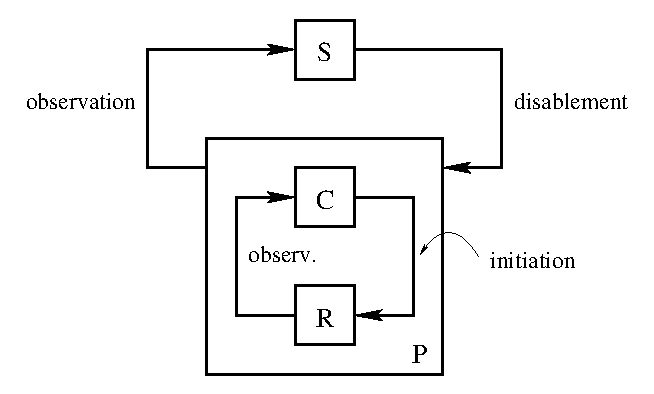
\includegraphics[scale=0.6]{figures/sup_plant}
  \caption{Supervisory control configuration.}
  \label{fig:sup_plant}
\end{figure}

The supervisor, S in Fig.~\ref{fig:sup_plant}, has to
prevent the plant from breaking the specification and from
getting blocked in a state from where it can not reach a
marked state by using as few restrictions on the plant as
possible. By observing the observable events of the plant
and disabling the controllable events of the plant, the
supervisor decides when, and if, it has to limit the
activity of the plant in order to keep the plant's behavior
within the specification. An important result of the
supervisory control theory is that such a supervisor can be
calculated from the models of the plant and specification so
that
$$S||P'$$
gives the system behavior.

In cases when there are several plant models $P_1,..,P_n$
with given specification models $Sp_1,...,Sp_n$ the
supervisor can also be generated and
$$S||P_1||...||P_n$$
gives the system behavior within specification.

Thus to control the system so that it satisfies the
specification, the synchronous composition of the plant and
supervisor models has to be implemented in the control
software. Using the conventional implementation methods,
i.e. implementing the synchronization using PLC programming
techniques, the solution becomes complex which makes it
difficult to distribute across multiple control computers.
Next section presents an example illustrating how the
synchronous composition can be implemented using the new
standard.

\section{Synchronization: An Example}
\label{sec:example}
In previous section it is shown that the synchronization
operator is a central concept for the results of supervisory
control theory. Now an example is presented showing how that
theoretical concept can be implemented using IEC 61499
function blocks for a small system before a general method
is given.

Consider a system containing two plants, \texttt{P1} and
\texttt{P2}, shown in Fig.~\ref{fig:plants}.These plant
models may represent two manufacturing resources with a
1-place buffer in-between. All events in the models are
controllable and observable. The desired behavior of the
system is that event \texttt{b} must always precede event
\texttt{c}, which means that a product must leave buffer
before another one can enter. The supervisor for this
specification can be generated and is shown in
Fig.~\ref{fig:sup}. In cases where the specification is
more complex it needs to be modeled using the automaton and
provided for the supervisor generation.
\begin{figure}[b]
  \centering 
  \fig[scale=0.55]{\texttt{P1}}{figures/P1_aut} 
  \fig[scale=0.55]{\texttt{P2}}{figures/P2_aut}
  \caption{Discrete event models of the plants.}
  \label{fig:plants}
\end{figure}
\begin{figure}[b]
  \centering 
  \fig[scale=0.55]{\texttt{S}}{figures/Sp_aut}
  \caption{The model of the supervisor.}
  \label{fig:sup}
\end{figure}
\begin{figure}[t]
  \centering 
  \fig[scale=0.45]{\texttt{SYS}}{figures/Sys_aut}
  \caption{The model of possible system behavior while satisfying
    the desired system behavior, $S||P_1||P_2$.}
  \label{fig:sys}
\end{figure}
Full synchronous execution of these models gives the system
that behaves as freely as possible while fulfilling the
specification. The resulting model of the system is shown in
Fig.~\ref{fig:sys}.

% IEC 61499 intro
The emerging standard IEC 61499 specifies a generic
architecture for measurement and control of industrial
processes. The architecture is based on functional software
units called function blocks. The most common type of
function block in an application is basic function block and
it is shown in Fig.~\ref{fig:61499_intro} using the
graphical representation. This type of block executes
algorithms based on the arriving events and generates new
events that are passed on when the algorithms finish
execution. The algorithms use data associated with incoming
events to update the internal variables and produce the
output data associated with the outgoing events. Which
algorithms are invoked is controlled by the execution
control chart (ECC) which is an automaton with algorithms
associated with different states. When a state is entered
the algorithms associated with it are executed once and the
ECC stays in the state until a condition for leaving is
fulfilled. The conditions upon which transitions occur are
boolean expressions involving event input variables,
internal variables, input variables, and output variables.
When the expression evaluates to \texttt{true} the
transition occur. Special case is transition labeled with
\texttt{1}, it is taken as soon as the algorithms finish
execution.
\begin{figure}
  \centering
  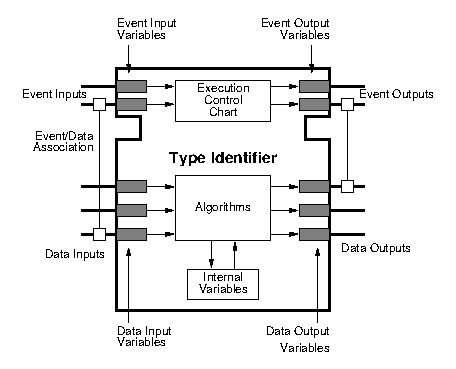
\includegraphics[scale=0.4]{figures/basic_block}
  \caption{Anatomy of a basic function block type.}
  \label{fig:61499_intro}
\end{figure}

Function block types that generate the behavior of the plant
and supervisor models for the example are shown in
Fig.~\ref{fig:systemFBs}. The event input of each block
type is \texttt{OCCURRED}. It signals that an discrete event
has occurred and that the model should update its state
according to the data inputs. The data inputs are boolean
variables representing the discrete events in the model's
alphabet. For well defined behavior only one of the data
inputs associated with the \texttt{OCCURRED} event must be
\texttt{true} when the event is received. The model's state
is then updated according to the discrete event that this
data input represents and the event output \texttt{DONE} is
generated. It signals that the model has updated its state
and that the data outputs are ready. The data outputs are
boolean variables representing the enabled events after the
model has updated its state, i.e. the events labeling the
transitions that are possible from the new state.

The function block type that is generated according to the
new method presented is shown in Fig.~\ref{fig:syncFB} and
is called synchronization function block type. The data
inputs and outputs of the block type are application
specific, since they are defined by the models that will be
synchronized. The event input and output, on the other hand,
are the same for all applications which also makes the ECC
of the block type the same for all applications. The ECC for
the block type is shown in Fig.~\ref{fig:ecc_sync}. The
\texttt{DISABLE\_EVENTS} algorithm associated with the
\texttt{SYNC} state is where the synchronized execution is
implemented. The \texttt{UPDATE} event is sent as soon as
the \texttt{DISABLE\_EVENTS} algorithm has finished
execution.

\begin{figure}
  \centering
  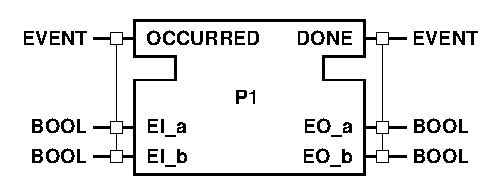
\includegraphics[scale=0.5]{figures/P1}\\(a)
  \vskip 5mm
  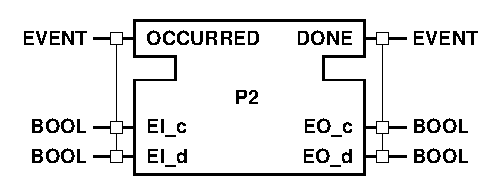
\includegraphics[scale=0.5]{figures/P2}\\(b)
  \vskip 5mm
  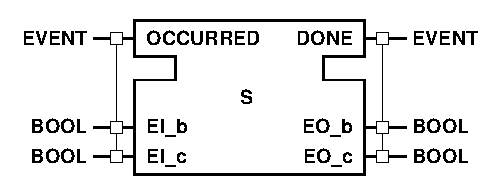
\includegraphics[scale=0.5]{figures/Sp}\\(c)
  \caption{The function block types implementing (a)
    plant 1, (b) plant 2, and (c) supervisor.}
  \label{fig:systemFBs}
\end{figure}
\begin{figure}
  \centering
  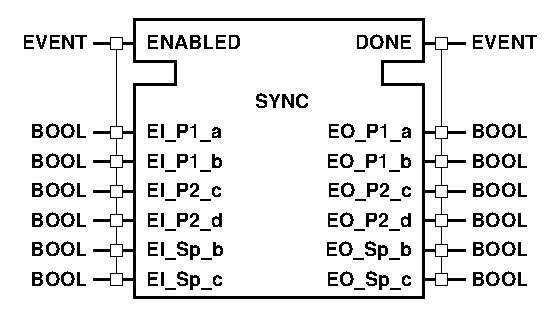
\includegraphics[scale=0.5]{figures/SYNC}
  \caption{The function block type for the synchronization.}
  \label{fig:syncFB}
\end{figure}
\begin{figure}
  \centering
  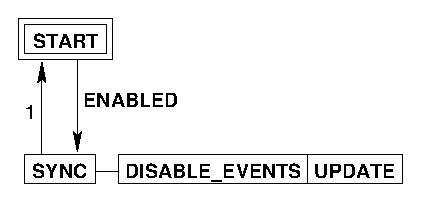
\includegraphics[scale=0.6]{figures/sync_ecc}
  \caption{The execution control chart for the
    synchronization function block type.}
  \label{fig:ecc_sync}
\end{figure}

The synchronization block reads the enabled events of the
synchronized models and disables the events that are not
enabled in all the models that have that event in their
alphabets. Each boolean data input signals if the event in
the model represented by that input is enabled
(\texttt{true}) or disabled (\texttt{false}). By setting the
corresponding data output to \texttt{false} the
synchronization block signals that the transition labeled by
that event is not allowed to occur in the model during the
next update cycle. To calculate each data output a logical
expression consisting of all data inputs that represent the
same event, connected by logical \texttt{and} operation, is
used. This means that if the event is enabled in all of the
models that have the event in their alphabet it is allowed
to occur in the next update cycle. Otherwise the expression
is false and the event is disabled. Following implementation
of the \texttt{DISABLE\_EVENTS} algorithm in IEC 61131
structured text does the computation:
\begin{verbatim}
EO_P1_a := EI_P1_a;
EO_P1_b := EI_P1_b AND EI_S_b;
EO_P2_c := EI_P2_c AND EI_S_c;
EO_P2_d := EI_P2_d;
EO_S_b := EI_P1_b AND EI_S_b;
EO_S_c := EI_P2_c AND EI_S_c;
\end{verbatim}
Since the event \texttt{a} is in the alphabet of the
\texttt{P1} model only, it is always allowed to occur if it
is enabled. The event \texttt{b} is allowed to occur in
\texttt{P1} model only if it is enabled in \texttt{P1} and
\texttt{S} models at the same time since it is contained in
both alphabets. The same applies to the event \texttt{b} in
\texttt{S} model, hence the same logical expression. Events
\texttt{d} and \texttt{c} are treated in the same manner.

The control application connecting all of the function
blocks together is shown in Fig.~\ref{fig:app}. Small
circles in the figure are event multiplexer and
demultiplexer. Event multiplexer generates an event on the
output every time an event arrives at any one of the inputs.
Event demultiplexer does the opposite and generates an event
on all of the outputs whenever an event arrives at the
input.
\begin{figure}
  \centering
  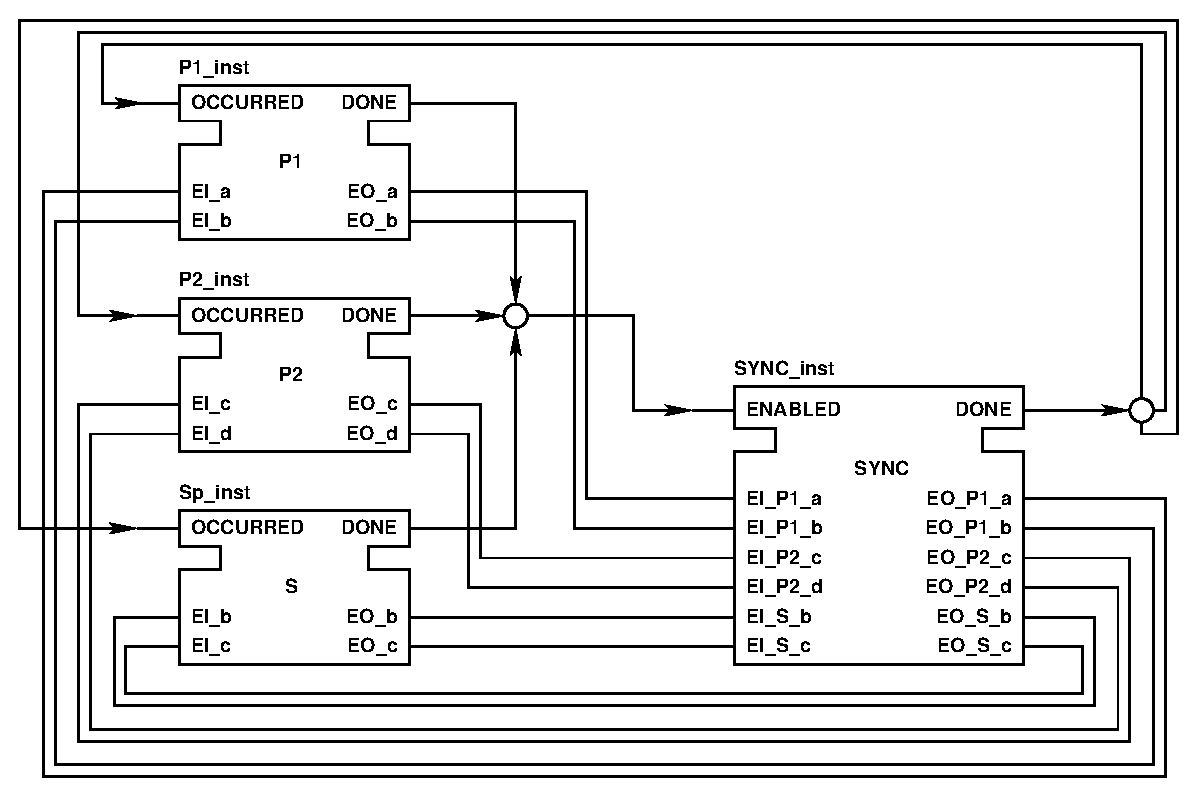
\includegraphics[scale=0.45]{figures/app}
  \caption{The control application for the example.}
  \label{fig:app}
\end{figure}

The method for generation of the \texttt{DISABLE\_EVENTS}
algorithm can be generalized for any number of models. This
general method is presented in the next section.

\section{Synchronization: General Approach}
The method for implementation of the full synchronous
composition for the general system containing any number of
discrete event models is made up of two major steps. The
first step is creation of the function block types that
generate the behavior of the discrete event models. The
interface that these blocks have to adhere to is shown in
Fig.~\ref{fig:model_interface}. These blocks are
application specific but they can be automatically generated
from discrete event models.

\begin{figure}[b]
  \centering
  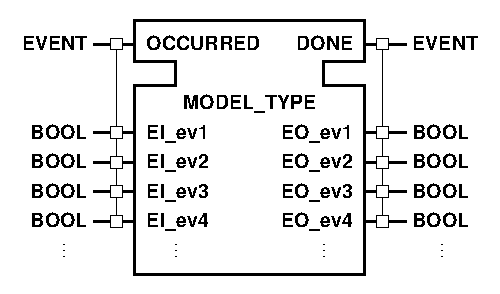
\includegraphics[scale=0.5]{figures/model_interface}
  \caption{The interface definition for the function block
    implementation of the discrete event models.}
  \label{fig:model_interface}
\end{figure}
\begin{figure}[t]
  \centering
  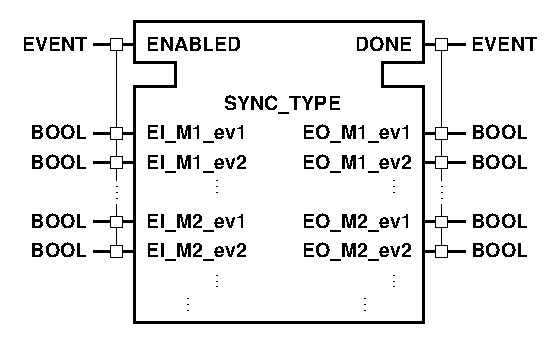
\includegraphics[scale=0.5]{figures/sync_interface}
  \caption{The interface definition for the synchronization
    function block type.}
  \label{fig:sync_interface}
\end{figure}

The second step is creation of the synchronization function
block type. The interface of this block is shown in the
Fig.~\ref{fig:sync_interface}. The execution control chart
for the function block type is the same as shown in
Fig.~\ref{fig:ecc_sync} since it is application generic.

The \texttt{DISABLE\_EVENTS} algorithm can be generated as
follows: Let $M$ be the set of all models for
synchronization. For all $m,e$ such that $m\in M$ and
$e\in\Sigma^m$:
\begin{equation}\label{eq:lexp}
  {\rm EO}\_m\_e:=\bigwedge_{\{n:n\in
    M\land e\in\Sigma^n\}}{\rm EI}\_n\_e
\end{equation}
The iteration over all events of all models is for the
generation of the logical expression assignments for all
data outputs, which are represented by EO\_$m$\_$e$. The
right hand side of~(\ref{eq:lexp}) generates the logical
expression that covers all the cases of the synchronization
definition. The first case in~(\ref{eq:delta}) is covered by
$e\in\Sigma^n$ and the data input being \texttt{false} which
gives that EO\_$m$\_$e$ is \texttt{false} and thus the event
is disabled. The first case in (\ref{eq:qi}) is covered by
$e\in\Sigma^n$ and the data input being \texttt{true}, and
the second case in (\ref{eq:qi}) is covered by
$e\notin\Sigma^n$.

To further illustrate how the general method is applied
refer to the \texttt{DISABLE\_EVENTS} algorithm of the
example in Section~\ref{sec:example}. First two lines are
generated for the \texttt{P1} model since it has two events
in its alphabet. The first event gives the left hand side of
the first line, \texttt{EO\_P1\_a}. The right hand side is
generated by iterating over all models and looking for the
event \texttt{a} in the alphabets. If the event is found the
boolean variable for that model's event is added to the
logical expression. In example, event \texttt{a} is found
only in model \texttt{P1} and therefore the right hand side
contains only variable \texttt{EI\_P1\_a}. The second event
of the model \texttt{P1} gives the left hand side of the
second line to be \texttt{EO\_P1\_b}. Looking for the event
\texttt{b} in the models it is found in \texttt{P1} and
\texttt{S} so the right hand side of (\ref{eq:lexp}) gives
\texttt{EI\_P1\_b AND EI\_S\_b}. Continuing this procedure
produces the whole \texttt{DISABLE\_EVENTS} algorithm in the
example.

When algorithm is generated what is left is to connect
instances of the model function blocks with the
synchronization function block to generate the control
application. Some further considerations for the
implementation of supervisory control theory are presented in
the following section.

\section{Applications in supervisory control theory}
\label{sec:app_SCT}
Since the general method presented is suitable for computer
implementation it is interesting to investigate how this
fact can ease the implementation of control applications
using supervisory control theory. 

Today implementation of a distributed control application is
done using application structure similar to the structure in
Fig.~\ref{fig:old_app_struct}. Supervisor \texttt{S} in
the application is manually crafted using informal
specifications of the system behavior, and transfered to the
PLC-code. For each application the communication between the
supervisor and the plants has to be implemented in a
application specific way since the existing standards for
communication between PLCs are at a low level of
abstraction. Using IEC 61499 the communication part of the
application is abstracted far away from the hardware level
and the control engineer is only considering the event and
data passing between the functional parts of the
application, i.e. function block instances. When the system
plants are upgraded or changed the procedure of supervisor
crafting has to be done once again and very small parts of
the code from the application already implemented are
reused, i.e. the communication parts.
\begin{figure}
  \centering 
  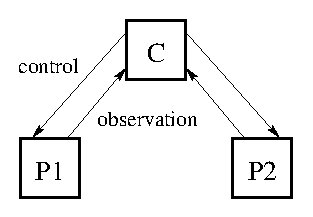
\includegraphics[scale=0.6]{figures/old_app_struct}
  \caption{The structure of distributed control applications today.}
  \label{fig:old_app_struct}
\end{figure}

In software tool Supremica \cite{aff:sup:2003,www:sup:2004},
algorithms from supervisory control theory are implemented
so that a supervisor can be synthesized from automata models
of the plants and specifications. The algorithm that
implements the general method for synchronization according
to this paper is also implemented in the same tool. What
this means is that the control engineer can focus on the
correct modeling of the plants and transferring of the
informal specifications to the specification models for use
in the Supremica tool. Then the tool automatically generates
the supervisor in form of an automaton model, function block
types that implement the skeleton for the plants, the
supervisor automaton, synchronous composition function block
and finally the control application that connects the
instances of the generated function block types as seen in
Fig.~\ref{fig:app} for the example. The skeleton in this
case refers to the fact that the communication with the
hardware has to be implemented by hand but all the behavior
of the models is automatically generated. Using the tool to
generate the control application gives new application
structure as shown in Fig.~\ref{fig:new_app_struct}. In
this structure, only the models for the generation of the
plant blocks and the hardware control portion of those
blocks have to be upgraded whenever the plants in the system
change. All other parts of the application are regenerated
automatically.
\begin{figure}[b]
  \centering 
  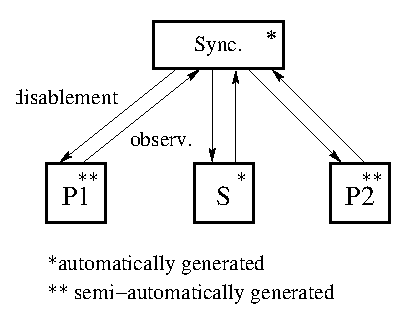
\includegraphics[scale=0.6]{figures/new_app_struct}
  \caption{A new structure for distributed control applications.}
  \label{fig:new_app_struct}
\end{figure}

When trying to implement the control application for complex
systems with many plants and specifications the problem of
state space explosion is encountered when trying to
synthesize the supervisor model. There are methods that
represent the plants, specifications and the supervisor in
different ways to try to cope with the problem. For example,
a supervisor may be expressed as a single automaton,
multiple automata, and a binary decision diagram for
off-line synthesis. Or the supervisor may be synthesized
on-line while the control application is executing. The
method presented in this paper can be used for
synchronization of all types of representations since the
model interface (see Fig.~\ref{fig:model_interface}) is
based on events which are a general characteristic of the
discrete event models.

\section{Conclusion}
Using supervisory control theory in construction of control
applications can significantly reduce development time but
until now it was difficult to apply the theory to
implementation of distributed control applications. Using
the emerging standard IEC 61499 it becomes significantly
easier. The method presented in this paper brings
supervisory control theory together with distributed control
application development in an efficient way.

Since the method is implemented in the Supremica tool it
significantly contributes to the shorter control application
development time since it is a part in automatic generation
of control applications. The method is also future proof by
using an inherent characteristic of discrete event models
for the interface upon which synchronization function block
is generated.

The method and function block programming in general can be
tested using the Function Block Development Kit (FBDK),
\cite{c:fun:2002}. For further information about IEC 61499
function blocks see \cite{c:ope:2002}.

\bibliography{/home/cengic/research/Bibliographies/desbib.bib}

\end{document}

